\documentclass[10pt,a4paper]{article}
\usepackage[utf8]{inputenc}
\usepackage[french]{babel}
\usepackage{listings}
\usepackage{graphicx}
\usepackage[left=2cm,right=2cm,top=2cm,bottom=2cm]{geometry}
\usepackage{hyperref}
\usepackage{amsmath,amssymb}
\usepackage{fontawesome}
%opening
\title{Revision}
\author{Nicolas Vadkerti}
\usepackage{listings} % Required for inserting code snippets
\usepackage[usenames,dvipsnames]{color} % Required for specifying custom colors and referring to colors by name

\definecolor{DarkGreen}{rgb}{0.0,0.4,0.0} % Comment color
\definecolor{highlight}{RGB}{255,251,204} % Code highlight color

\lstdefinestyle{Style1}{% Define a style for your code snippet, multiple definitions can be made if, for example, you wish to insert multiple code snippets using different programming languages into one document
language=Perl, % Detects keywords, comments, strings, functions, etc for the language specified
backgroundcolor=\color{highlight}, % Set the background color for the snippet - useful for highlighting
basicstyle=\footnotesize\ttfamily, % The default font size and style of the code
breakatwhitespace=false, % If true, only allows line breaks at white space
breaklines=true, % Automatic line breaking (prevents code from protruding outside the box)
captionpos=b, % Sets the caption position: b for bottom; t for top
commentstyle=\usefont{T1}{pcr}{m}{sl}\color{DarkGreen}, % Style of comments within the code - dark green courier font
deletekeywords={}, % If you want to delete any keywords from the current language separate them by commas
%escapeinside={\%}, % This allows you to escape to LaTeX using the character in the bracket
firstnumber=1, % Line numbers begin at line 1
frame=single, % Frame around the code box, value can be: none, leftline, topline, bottomline, lines, single, shadowbox
frameround=tttt, % Rounds the corners of the frame for the top left, top right, bottom left and bottom right positions
keywordstyle=\color{Blue}\bf, % Functions are bold and blue
morekeywords={}, % Add any functions no included by default here separated by commas
numbers=left, % Location of line numbers, can take the values of: none, left, right
numbersep=10pt, % Distance of line numbers from the code box
numberstyle=\tiny\color{Gray}, % Style used for line numbers
rulecolor=\color{black}, % Frame border color
showstringspaces=false, % Don't put marks in string spaces
showtabs=false, % Display tabs in the code as lines
stepnumber=5, % The step distance between line numbers, i.e. how often will lines be numbered
stringstyle=\color{Purple}, % Strings are purple
tabsize=2
}

\newcommand{\insertcode}[2]{\begin{itemize}\item[]\lstinputlisting[caption=#2,label=#1,style=Style1]{#1}\end{itemize}} 

\newcommand{\reels}{\mathbb{R}}
% \insertcode{"Scripts/example.pl"}{Nena would be proud.} 

\begin{document}

\maketitle
\section{Notation}

 \begin{equation}\label{xx}
\begin{split}
&f = [ \reels^{*}_{+}\Rightarrow\reels] \\
&x\ \mapsto \ln(x)\\
\end{split}
\end{equation}
\subsection{Les Ensemles}
Notation pour les ensembles \\
$\reels \rightarrow $les\ reel\\
$\reels^{*}\rightarrow $Tous\ sauf\ 0 \\
$\reels^{*}_{+} \rightarrow $Tous\ les\ reels\ positif\ sauf\ 0 \\
$A\cap B \rightarrow  $Tous\ les\ nombres\ dans\ l'ensembles\ A et B en même temps\\
$A\cup B \rightarrow$ Tous les nombres compris dans A et B 
\begin{figure}[h!]
\centering
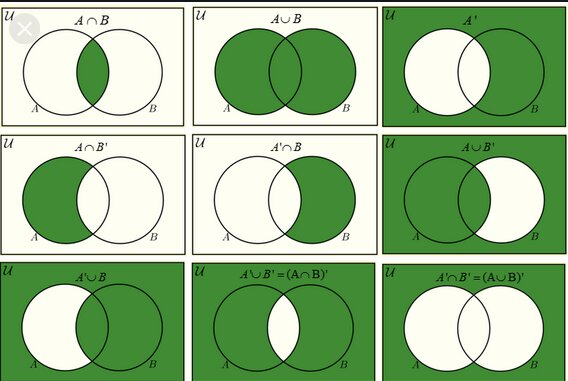
\includegraphics[scale=0.30]{image/ensemble.jpg}
\caption{Ensembles}
\label{fig:net}
\end{figure}\\
$\forall \rightarrow$ Pour tous\\
$\exists \rightarrow$ Il existe\\
$\Rightarrow\rightarrow$ ``implique'' : Si A est Vrai alors B est vrai, donc si A Faux, alors B aussi\\
$\Leftrightarrow \rightarrow$ equivalence : Si A $\Leftrightarrow$ B alors A$\Rightarrow$ B et B$\Rightarrow$A
\section{Fonctions Références}
\begin{itemize}
 \item ln, log(x)\\
 $\ln(e)=1$\\
$\ln(1)=0$\\
$\ln(x.y)=ln(x)+ln(y)\Rightarrow\ln(x^y)=y\ln(x)$\\
 
$log_{10}(x)=\frac{ln(x)}{ln(10}$\\
Exemple:\\
$log_{10}(1000)=log_{10}(10^3)=3\frac{ln(10)}{ln(10)}=3$\\
 
 \item exp(x)\\
$e^{x+y}=e^x.e^y$\\
$ln(e^x)=x$ 
 \item sin, cos, tan
 \item Les polynomes \\
\begin{equation}\label{xx}
\begin{split}
&f(x)=x^2+x+n\\
\end{split}
\end{equation}
\item La fonction inverse : $\frac{1}{x}$
\item Les Equations Linaires
\end{itemize}





\section{Les équations Linéaires}
 \begin{equation}\label{xx}
\begin{split}
&f = [ \reels\rightarrow\reels] \\
&x\ \mapsto ax+b \\
\end{split}
\end{equation}
\begin{figure}[h!]
\centering
\includegraphics[scale=0.0250]{image/lineaire.jpg}
\caption{Interprétation Graphique}
\label{fig:net}
\end{figure}

% $$\left|\begin{array}{l}a_x\\a_y\\a_z\end{array}\right.=\left|\begin{array}{l}0\\-g\\0\end{array}\right.$$
% \begin{equation}
%    &f[\reel^{*}{+}\to\reel]
%   &x\mapto \ln(x) 
% \end{equation}


\section{Les identités remarquables}
\begin{itemize}
 \item $(a+b)^2= a^2+b^2+ 2ab$
 \item $(a-b)^2 =a^2+b^2-2ab$
 \item $(a+b)(a-b) = a^2-b^2$
\end{itemize}
\section{Resolution de polynomes de degré 2}
\subsection{Méthode}
$f(x)=ax^2+bx+c$\\
Calcul du $\Delta $:\\
$b^2-4ac$\\
Si $\Delta <0$ L'equation n'admet aucune soltion dans $\reels$\\
Si $\Delta =0$ L'equation admet comme unique solution $x=\frac{-b}{2a}$\\
Si $\Delta >0$ L'equation 2 solutions $x^1$ et $x^2$ où $x^1= \frac{-b+\sqrt[]{\Delta}}{2a}$ et $x^2= \frac{-b-\sqrt[]{\Delta}}{2a}$ 
\begin{figure}[h!]
\centering
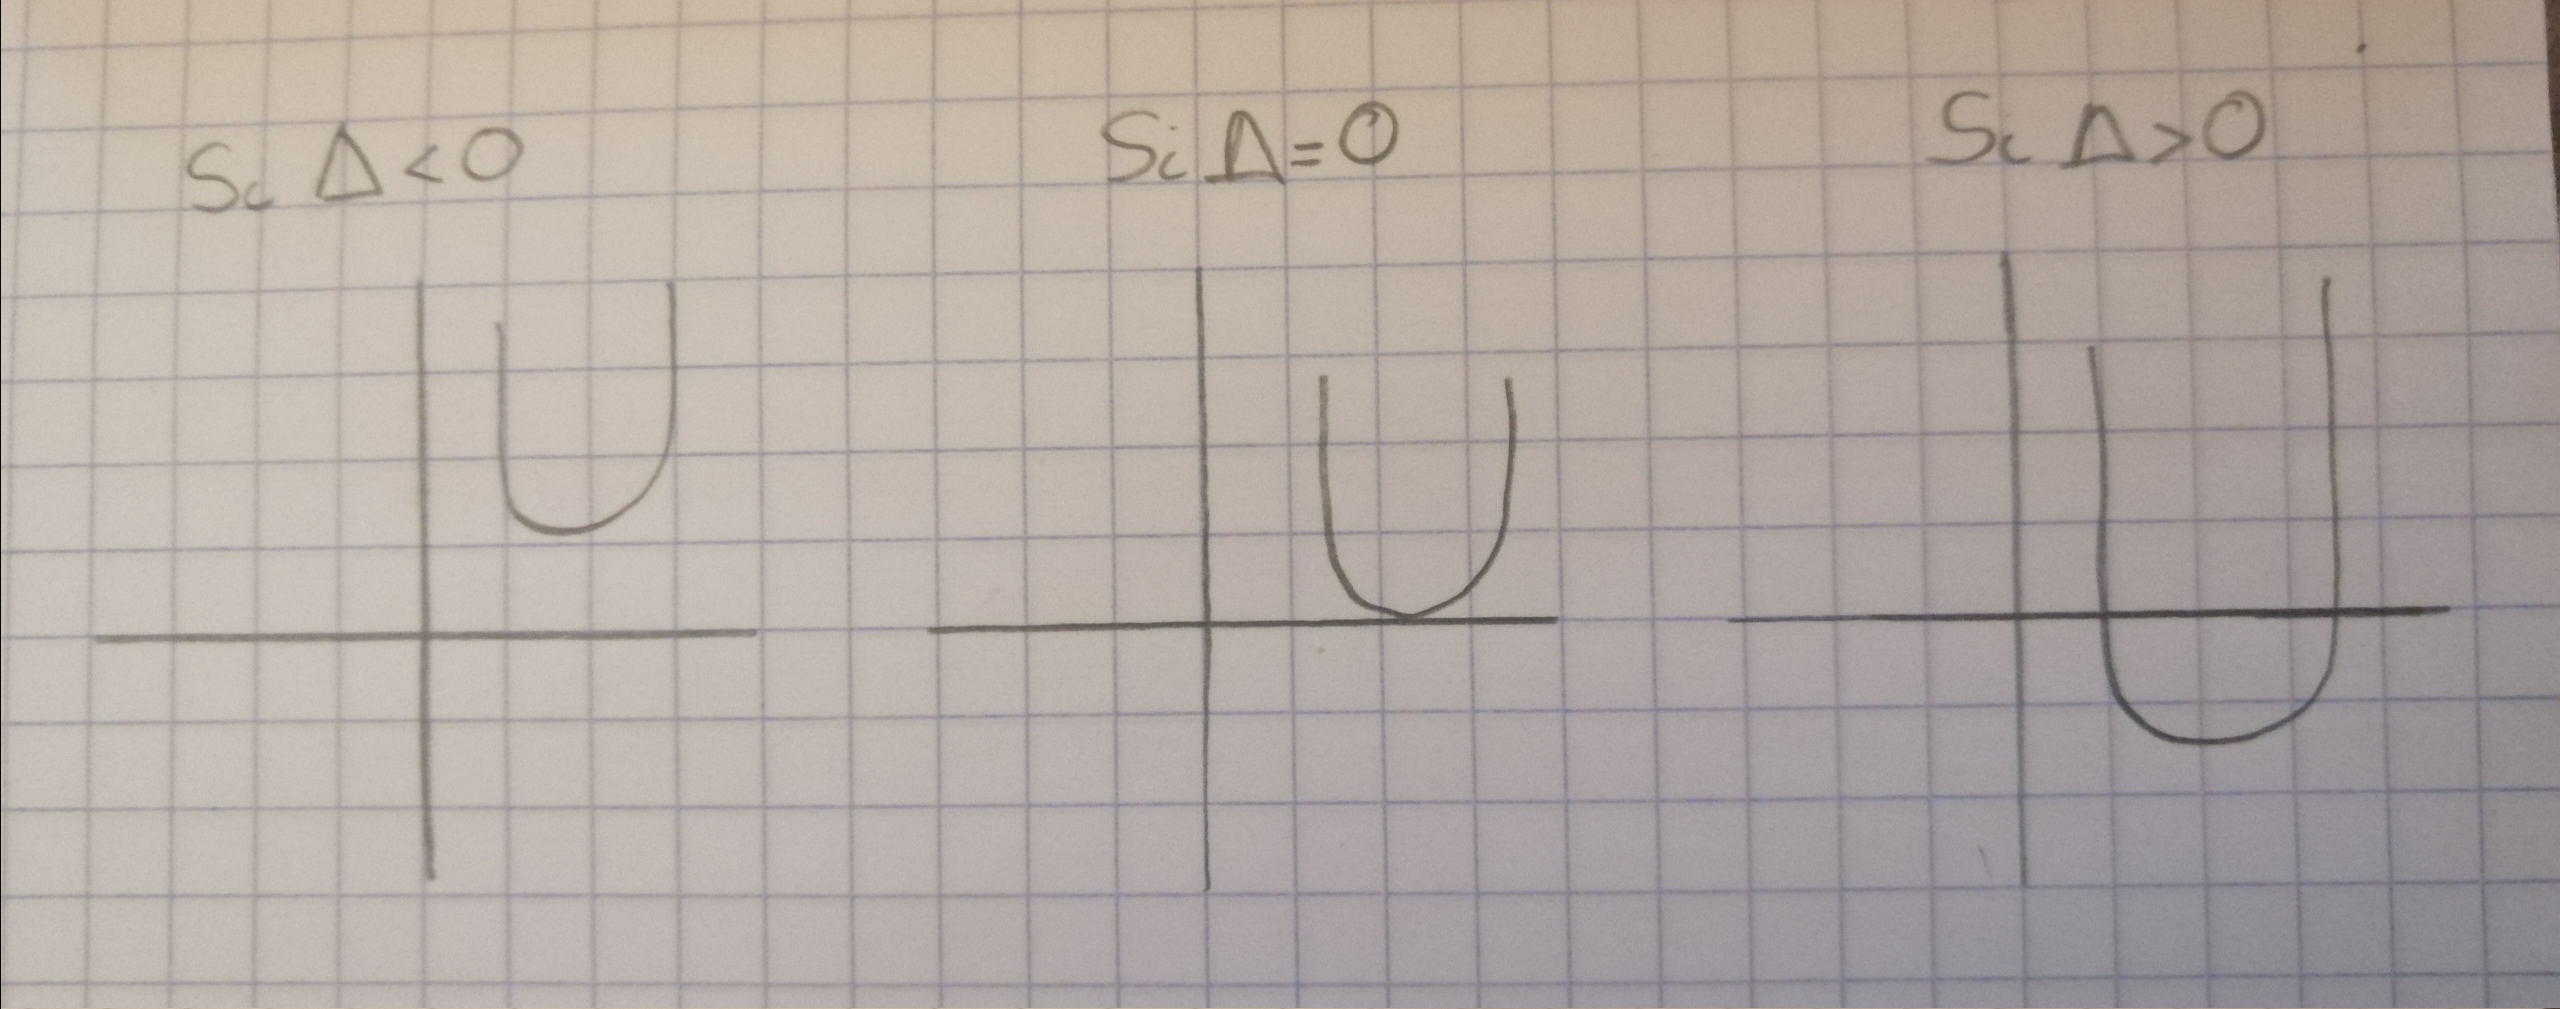
\includegraphics[scale=0.150]{image/poly.jpg}
\caption{Interprétation Graphique}
\label{fig:net}
\end{figure}
\newpage


\section{Les Puissances }
$a^x . a^y =a^{x+y}$ \\
\faExclamationCircle $\ a^x+a^y\neq a^{x+y} $\\

\section{La trigonometrie}
 \begin{figure}[h!]
 \centering
 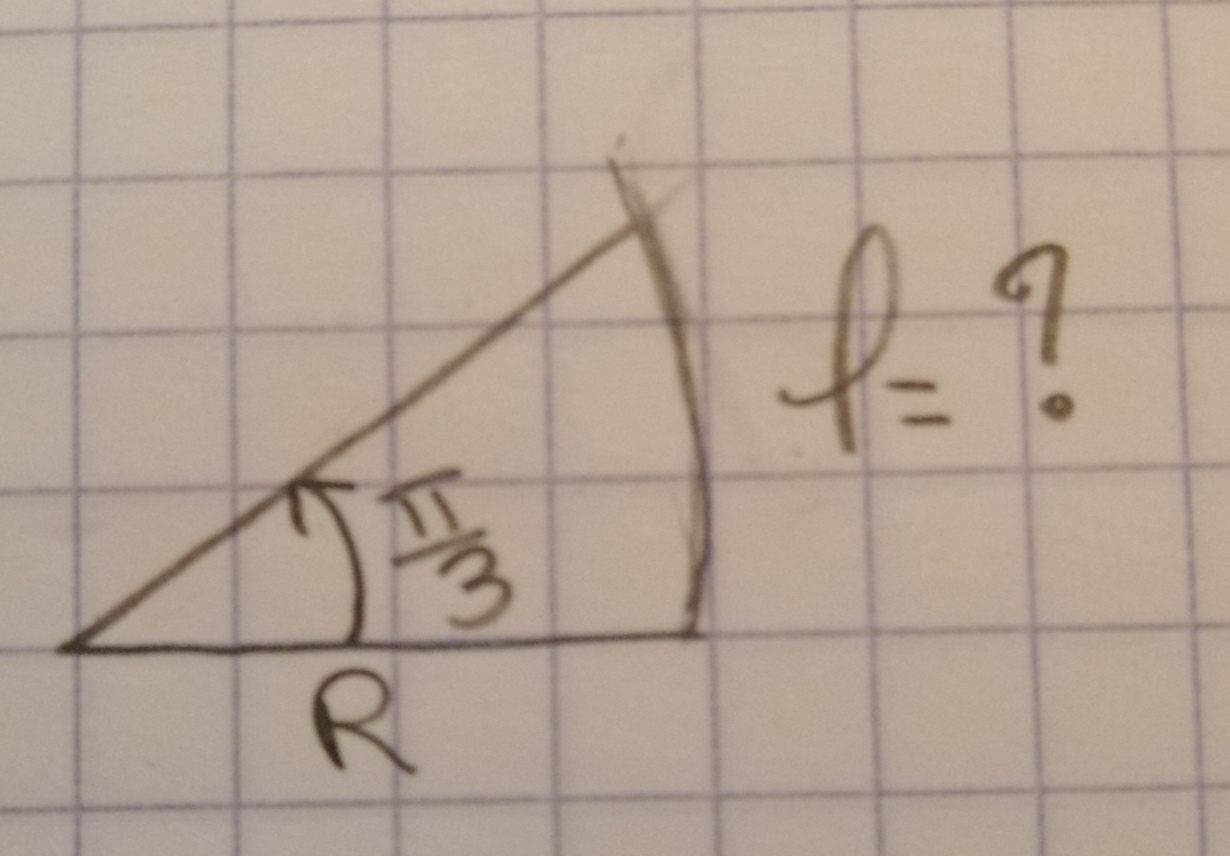
\includegraphics[scale=0.150]{image/trigo1.jpg}
 \caption{}
 \label{fig:net}
 \end{figure}

$l=\frac{\pi}{3}.R$\\
donc $l=angle.rayon$
\subsection{Le cercle unitaire}
Definition: Un cercle de rayon 1\\
 \begin{figure}[h!]
 \centering
 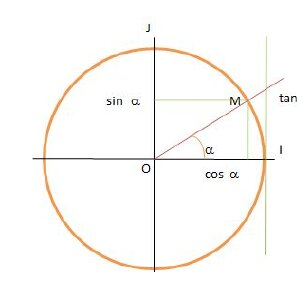
\includegraphics[scale=0.50]{image/trigo2.jpg}
 \caption{Le cercle unitaire}
 \label{fig:net}
 \end{figure}
 \subsection{Formule de trigonometrie}
 Formule à connaitre!!!!! (cahsohtoa)\\
 \begin{itemize}
 \item  $cos(\theta)=\frac{adj}{hyp}$\\
 \item $sin(\theta)=\frac{opp}{hyp}$\\
 \item $tan(\theta)=\frac{sin(\theta)}{cos(\theta)}=\frac{opp}{adj}$
 \end{itemize}

 
 \begin{figure}[h!]
 \centering
 \includegraphics[scale=0.10]{image/trigo3.jpg}
 \caption{Le cercle unitaire}
 \label{fig:net}
 \end{figure}

\subsection{Les valeurs Importants}
   \begin{figure}[h!]
 \centering
 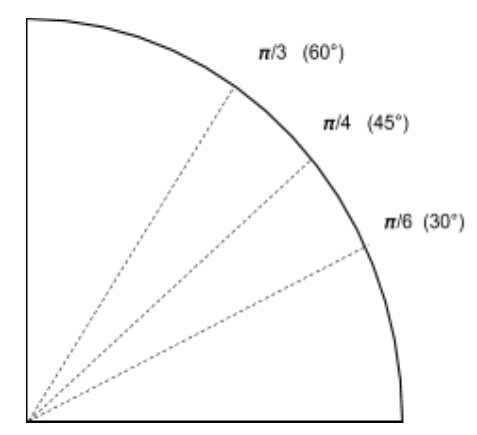
\includegraphics[scale=0.250]{image/trigo4.jpg}
 \caption{Valeurs à connaitre}
 \label{fig:net}
 \end{figure}

 
 
 
 \begin{center}
  \scalebox{3}{
\begin{tabular}{|l|l|l|}
\hline
   \  & cos & sin \\ \hline
    0 & 1  & 0 \\ \hline
    $\frac{\pi}{6}$ & $\frac{\sqrt{3}}{2}$  & $\frac{1}{2}$\\ \hline
    $\frac{\pi}{4}$ & $\frac{\sqrt{2}}{2}$  & $\frac{\sqrt{2}}{2}$\\ \hline
    $\frac{\pi}{3}$ &$\frac{1}{2}$& $\frac{\sqrt{3}}{2}$\\ \hline
    $\frac{\pi}{2}$ & 0 & 1 \\ \hline 
\hline
\end{tabular}}
 \end{center}
 
 
 Les valeurs des tangentes sont facile à retrouver grâce à $\frac{sin(\theta)}{cos(\theta)}=tan(\theta)$
 \subsection{Les formules de trigonometrie volume 2}
 $cos(a+b)=cos(a).cos(b)-sin(a)sin(b)$ (``coco''  moins ``sisi'')\\
 $sin(a+b)= sin(a).cos(b) + cos(a).sin(b)$ (``sico'' plus ``cosi'')\\
 -----\\
$cos(a-b)=cos(a).cos(b) + sin(a)sin(b)$ (avec le cos, le signe change, pas la fonction)\\
$sin(a-b)= sin(a).cos(b) - cos(a).sin(b)$(avec le sin, le signe change pas, mais la fonction oui) \\
 \section{La formule d'Euler (De l'air)}
 Wikipedia nous dit:  Les formules d'Euler relient les fonctions trigonométriques à l'exponentielle complexe. Ces formules permettent de linéariser cos(nx) et sin(nx), c'est-à-dire d'exprimer ces quantités en fonction de cos(px) et sin(px).\\
$cos(\theta)=\frac{e^{i\theta}+e^{-i\theta}}{2}$\\
$sin(\theta)=\frac{e^{i\theta}-e^{-i\theta}}{2i}$
 
 Si on veut dévelloper : $cos^4(\theta)=\frac{(e^{io}+e^{-io})^4}{16}$
 \subsection{Comment dévelloper $(a+b)^n$}
 Deja, on prend le triangle de Pascal :\\
 1 (n=0)\\
 11(n=1)\\
 121(n=2)\\
 1331(n=3)\\
 14641(n=4)\\
 Puis par construction on peut ecrire pour n = 4 par exemple : $1a^?b^? + 4a^?b^? + 6a^?b^?+4a^?b^?+1a^?b^?$\\
 Pour déterminer les puissances rien de plus simple :  $1a^{n}b^{n-n} + 4a^{n-1}b^{n-(1+n)} + 6a^{n-2}b^{n-(n+2}+4a^{n-3}b^{n-(n+3)}+1a^{n-4}b^{n-(n+4)}$\\
 donc dans les faits on a: $a^4+4a^3b+6a^2b^2+4ab^3+b^4$
 \newpage
 \subsection{On revient à $cos^4(\theta)=\frac{(e^{io}+e^{-io})^4}{16}$}
$cos^4(\theta)=\frac{(e^{i\theta})^4+4(e^{i\theta})^3(e^{-i\theta})^1+6(e^{i\theta})^2(e^{-i\theta})^2+4(e^{i\theta})^1(e^{-i\theta})^3+(e^{-i\theta})^4}{16}$\\

 $=\frac{1}{8}cos(4\theta)+\frac{6}{16}+\frac{4}{8}cos(2\theta)$\\
 
 $\frac{1}{8}cos(4\theta)+\frac{3}{8}+\frac{1}{2}cos(2\theta)$
 
 
\end{document}


